\graphicspath{{chapters/notes/08/images/}}
\chapter{Liquid biopsies in oncology}
It is more feasible to track the tumor progression stage for a patient from liquid biopsies (panoramic overview at a time point), rather than from tissue biopsy (highly accurate snapshot in a specific site at a timepoint). How accurate can a liquid biopsy is depends on many factors: if there is homogeneity the quality is really similar to tissue biopsy. We might have different representations according to sites. The major advantage of liquid biopsy is being minimally invasive. Furthermore, it is easier for early diagnostics (screening), quantify the presence of minimal residual of disease.

\section{General considerations}
The main difference between tissue and liquid biopsies are listed in table \ref{tab:diff1}.
\begin{table}[H]
\centering

\begin{tabular}{ | p{4cm} | p{9cm} | }
 \hline
 \textbf{Tissue Biopsy} & \textbf{Liquid Biopsy} \\
 \hline
 \hline
 Accurate and detailed view of one tissue only & Landscape overview, with resolution depending on tumor burden, releasing rates, metastases and tumor heterogeneity. It is possible to get an aggregated signal of different tumor cell populations \\
 \hline
 Single tumor & Possibility of getting signal from multiple tumor masses \\
 \hline
 Signal relative to a specific point in time & At a certain point in time, but multiple serial samples can be collected \\
 \hline
 Invasive and painful for the patient, not feasible for all the tissues or in presence of metastatic sites & Minimally invasive (so it is possible to collect samples multiple times) and can be coupled with a routine blood draw \\
 \hline
 & It is possible to design specific assays to detect minimal quantities of tumor cells, for example the ones left behind after surgery. This is useful to detect minimal residual disease (MRD) and avoid tumor recurrence \\
 \hline
 & The collection of serial samples allows for example to track clonal evolution of the tumor over time, to catch treatment resistances early on and to monitor the patient's response to the treatment \\
 \hline
 & It can be used for early detection of cancer, many studies are trying to reach this objective \\
 \hline
\end{tabular}
\caption{Main differences between tissue and liquid biopsy I.}
\label{tab:diff1}
\end{table}


Other consideration are reported in table \ref{tab:diff2}.

\begin{table}[H]
\centering

\begin{tabular}{ | p{8cm} | p{8cm} | }
 \hline
 Tissue biopsy & Liquid Biopsy\\
 \hline
 \multicolumn{2}{| c |}{Material availability} \\
 \hline
 From needle biopsies, biopsies, surgical resections (if some material is left after the clinical protocol and the patient agrees to a research protocol) & From circulating tumor cells, extracellular vesicles, cell-free DNA (the most interesting). In healthy donors there is ~4ng/ml cell-free DNA (below 10 anyway), in tumor patients ~100s ng/ml (but the range is really wide). The numbers are higher if the tumor is metastatic and the treatment is also very influential on the quantity of cfDNA. Tumor patients under treatment have cfDNA quantities comparable to healthy people. Anyway, cfDNA quantity is influenced by a number of factors in addition to cancers so it is not a good diagnostic feature by itself \\
 \hline
 \multicolumn{2}{|c|}{Tumor content} \\
 \hline
 Tumor content can be assessed with a microscope: the proportion of tumor cells compared to healthy cells is measured based on morphology with a simple staining of the tissue slide. So tumor content is assessed by counting cells and considering the magnification of the image. If subtyping is needed, a staining for markers is performed. Computational methods are also available & The fraction of circulating tumor DNA (ctDNA) is inferred with methods based on genomics (or possibly also methylation) \\
 \hline
 \multicolumn{2}{|c|}{Tumor ploidy/aneuploidy } \\
  \hline
 Tumor ploidy: assesed with cytogenetics, FISH, or from NGS data & Average ploidy: inferred computationally based on genomics but it is quite tricky \\
 \hline
\end{tabular}
\caption{Main differences between tissue and liquid biopsy I.}
\label{tab:diff2}

\end{table}


\section{Issues in the interpretation of cfDNA data}

\subsection{Normalization on tumor content}
When interpreting data from liquid biopsies, it is fundamental to contextualize a mutation after observing it.
In order to associate a particular mutation to a particular diagnosis, the signal has to be normalized based on tumor content.
Without normalization, tumor content is the most influential variable on the patient's prognosis and this can be misleading.
For example, one mutation could look like it is linked to a specific type of tumor when it is actually present in other types too, but it is not detected due to the low tumor content of some samples (example in figure \ref{fig:norm}).
For this reason not all the literature available about liquid biopsies is reliable: lack of normalization leads to completely wrong conclusions. This applies to all kinds of assays: from microarrays to the sequencing of extracellular vesicles. \\

\begin{figure}[H]
\centering
    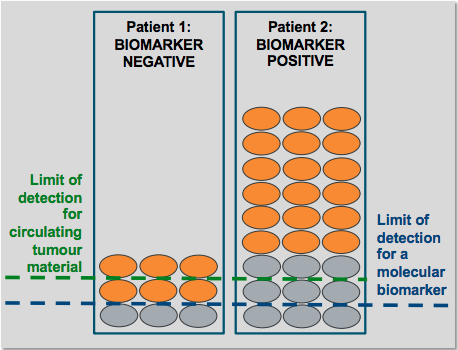
\includegraphics[width=0.4\linewidth]{norm.png}
    \caption{The two samples have the same percentage of tumor cells, however the first one results negative for the marker because of the low tumor content}
    \label{fig:norm}
\end{figure}

\subsection{Quantity of input material}
Another source of errors in the interpretation of cfDNA data is the amount of input material: if the patient's tumor content is high, the results could be obtained with a limited amount of extracted nucleic acid, but if the tumor content is low, too little material can lower the chances of detecting tumor cells (figure \ref{fig:quan}).
The problem is that in most cases the tumor content is unknown before the analysis and this must be considered when designing an experiment.
Usually the standard procedure is to begin with 2ml of plasma, the DNA content should be from 50 ng to 5ng.
If no tumor is detected, one should repeat the assay with more material (or sequence another vial and combine the results) to be sure that the tumor is not present and not just undetected.
In some cases some information about the state of the patient is available: for example if a patient is in remission more material is required.

Keep in mind that if the sample is pure, 10 ng of DNA should correspond to around 1500 diploid tumor genomes.

\begin{figure}[H]
    \centering
    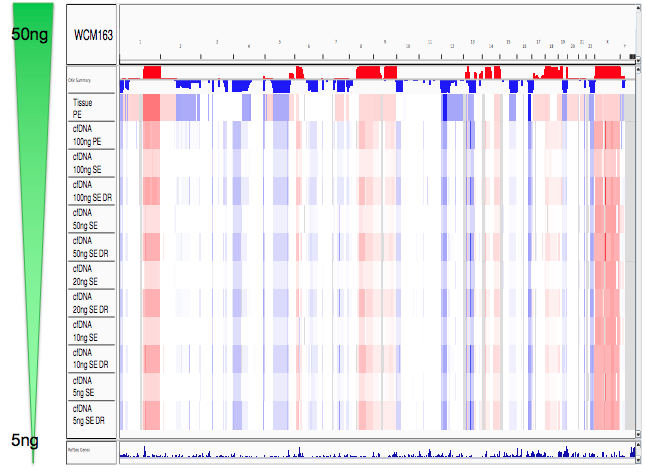
\includegraphics[width=0.5\linewidth]{quantity1.png}
    \caption{The same analyses are repeated with different quantities of starting material: for a patient with high tumor content the results do not change even with as little as 5ng of cfDNA}
    \label{fig:quan}
\end{figure}

\begin{figure}[H]
    \centering
    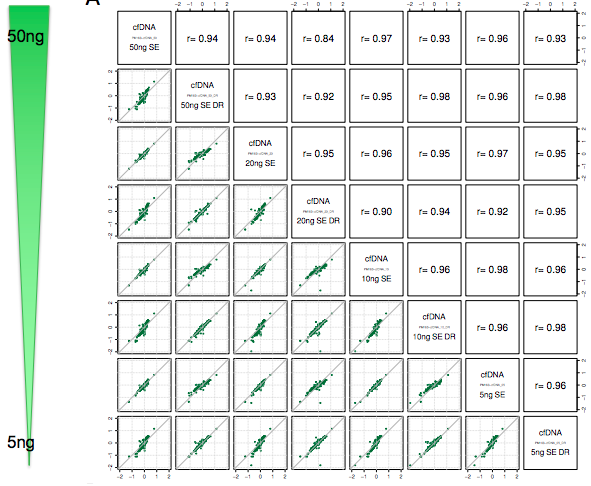
\includegraphics[width=0.7\linewidth]{quantity2.png}
    \caption{Copy number signal correlates very well between different initial amounts of cfDNA for a sample with high tumor content}
    \label{fig:quan2}
\end{figure}



\section{SNV detection in liquid biopsies}
Technical problems we have to face if we want to detect SNVs though liquid biopsies are:
\begin{itemize}
    \item PCR artifacts;
    \item Sequencing errors: one mutation should be validated by multiple reads to be confirmed;
    \item Problems related to the depth of coverage: the required coverage should be estimated considering the expected tumor content of the sample and deeper sequencing may be required;
\end{itemize}

But we also biological problems:

\begin{itemize}
    \item Low tumor content: ctDNA/cfDNA ratio
    \item Clonal hematopoiesis (when a hematopoietic stem cell starts making cells with the same genetic mutation): to distinguish the signal coming from clonal hematopoiesis, compare it with what has been sequenced before from solid tumors. It is rare to observe something in liquid biopsy that has never been noticed in solid ones.
    \item Copy number variations and ploidy: with a whole genome duplication and a SNV only present on one allele, the signal corresponding to the mutation is only 25\% and has to be correctly interpreted.
    \item \textbf{Intra-patient tumor heterogeneity}: very low allelic fractions for SNVs that are not clonal can be difficult to observe
\end{itemize}

Multiple \textbf{tools} are available to detect SNVs. Each tool will probably give different results (or partially concordant ones). Each tool can be tuned to favour some types of calls, so the tuning parameters should be carefully selected.

\section{Requirements depend on the application}

\begin{tabular}{ | p{6cm} | p{10cm} | }
 \hline
 \textbf{Application} & \textbf{Requirements} \\
 \hline
  Early tumor detection, MRD detection, Recurrence detection & Tumor quantity is low so a low signal is expected: higher quantity of starting material is required but there needs to be a 			balance between the number of false positives (with too much material) and false negatives (with too little) that can be produced \\
 \hline
	Tumor dynamics,Treatment response, Mechanisms of resistance & The assay should be designed in order to be able to distinguish between different clones (sub clonality analysis) \\
 \hline
 Single biomarker assessment & The only important thing is to detect whether one point mutation is present or not, so in this case tumor content is not important. A targeted assay is used and specific locations associated with the SNV are sequenced as deep as possible to detect the mutation \\
 \hline
\end{tabular}

\section{Whole genome vs targeted sequencing}
Whole genome sequencing has higher computational cost, while targeted assays have higher sample preparation time. The sequencing cost is higher for whole genomes but it does not decrease evenly \ref{fig:wg}.

\begin{figure}[H]
\centering
    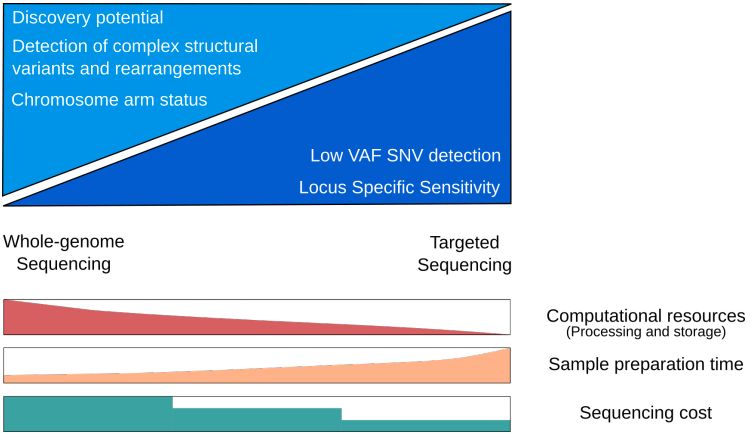
\includegraphics[width=0.6\linewidth]{wg.png}
    \caption{\label{fig:wg}Whole genome vs targeted sequencing}
\end{figure}

\section{Case studies}
\subsection{Case I}
Assay to study specific signal distribution for the disease of interest (prostate cancer). By analyzing this as a dynamic process, we might see the overall distribution of clonal DNA.
One of the lesion tracked was 21q22: the distribution on the top and the bottom are different at each time point with different dynamics. When the patient regressed 8p21, 21q22 emerged. Figure \ref{fig:case1}.

\begin{figure}
\begin{tabular}{cc}
  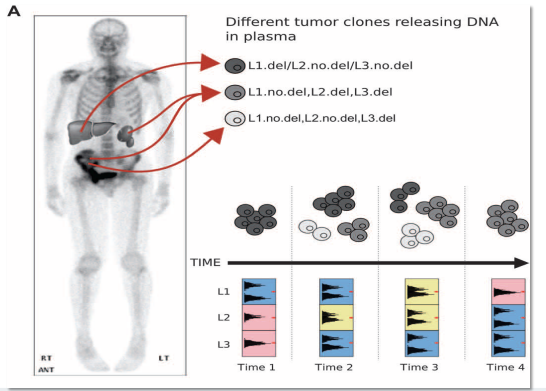
\includegraphics[width=0.4\linewidth]{case1a} &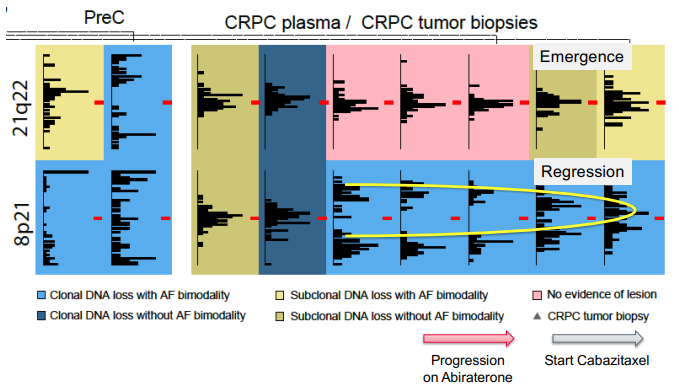
\includegraphics[width=0.6\linewidth]{case1b} \\
(a)  & (b)  \\
\end{tabular}
\caption{}
\label{fig:case1}
\end{figure}

\subsection{Case II}
Non-AR driven castration resistant prostate cancer, really rare as a de novo, but rising incidence especially after potent AR-pathway. Hard to treat and to diagnose.
Both tissue and liquid biopsy analysis to find:
\begin{itemize}
\item Potential biomarkers for liquid biopsy
\item Distinguish the transition to severe stage
\end{itemize}

First tissue heterogeneity study, see how similar metastases were. Resulting in homogeneity higher with the most aggressive phenotype (NE). The same was observed in liquid biopsy, confirming the potential NE biomarker usage. A liquid biopsy is identical to lymph node metastasis, very clear signal. In another patients, certain genes switch from one cluster to another from tissue to plasma, suggesting that the metastatic representation was partially heterogenous. We have a landscape overview.

\begin{figure}[H]
\centering
    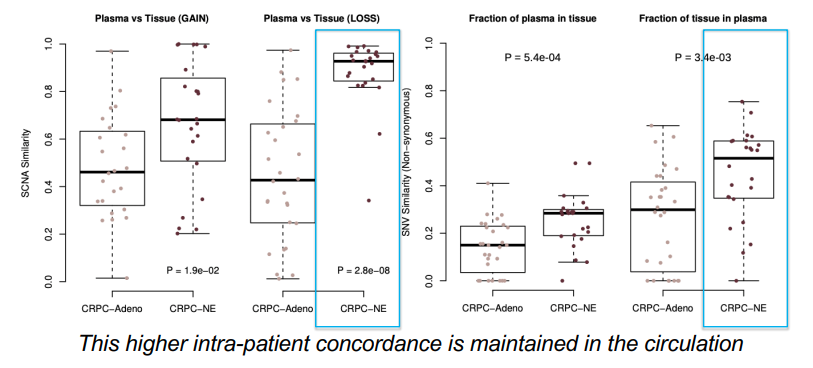
\includegraphics[width=0.7\linewidth]{case2.png}
    \caption{\label{fig:case2}Beltran, Romanel et al, JCI 2020}
\end{figure}

Man initially diagnosed with adenocarcinoma, switched to NE (clinical assessment). Plasma sample before NE diagnosis and multiple tissue biopsies. It was noted that the liver metastasis (NE) had lesion represented in the plasma sample, suggesting that a clone that was transforming was already present at past time. In certain cases, a liquid biopsy can be informative of something that would only emerge later clinically. \\

By comparing the genomic content of each metastasis with liquid biopsy, we can come up with a measure of the modification contributing more to the disease.


\section{Take-home message}
\textbf{Possible exam question}: what type of assay should be run and which are the requirements for a specific situation.
\subsection{Challenges in the tracking of tumor evolution}
\begin{itemize}
\item ctDNA content (fraction of tumor content in circulation)
\item polyploidy (allelic imbalance events)
\item ability to detect signal is gene region dependent and individual dependent
\item different DNA release rates form different metastases

\end{itemize}
\begin{figure}[H]
\centering
    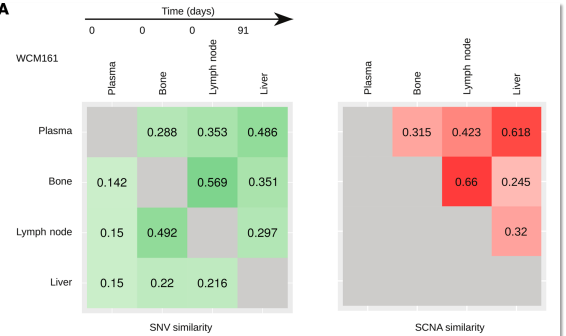
\includegraphics[width=0.7\linewidth]{time.png}
    \caption{xMetastatic biopsy time points during clinical progression
from CRPC-Adeno to CRPC-NE. Plasma sample at time of CRPCAdeno with lymph node and bone metastases displayed a genomic ctDNA profile most similar to the CRPC-NE liver metastasis observed on imaging and biopsied 3 months later at time of progression on abiraterone.}
\label{fig:norm}
\end{figure}


% #TODO MANCA LA PARTE DI QUANDO È ANDATA VIA A METÀ LEZIONE
